\documentclass[10pt]{article}
\usepackage{icmlko}

\icmlmeta{IP 파운데이션 월드모델}{141}{세 번째 누수는 시점이었다}{후보 축을 기간 갈라 다시 봤더니 숨은 것은 없었고, 대신 가드 둘을 다 통과하면서 쓰면 안 되는 축이 나왔다 --- 그리고 내가 사흘 전 헤드라인에 쓴 플래그가 그것이었다}

\begin{document}

\twocolumn[
\icmlheader

\begin{abstract}
노트 140이 ``전체 상관이 기간 구조를 숨긴다''를 보이고 후보 축 스물몇 개를
기간 갈라 재검토하라고 남겼다. 했다. \textbf{숨은 것은 없었다} --- 도메인
$\times$축 139쌍에서 ``전체는 약한데 두 기간 다 센'' 보석이 0개, ``전체는
센데 기간 부호가 반대인'' 덫이 0개다. $|\rho|$ 중앙값이 전체 0.065 · 이전
0.076 · 이후 0.076으로 거의 같다. \textbf{노트 140의 규약 권고를 그만큼
좁힌다} --- 전체 상관은 97\%의 경우 멀쩡한 요약이다. \textbf{그런데 그
훑기에서 다른 것이 나왔다.} \texttt{kitsu\_rank}와
\texttt{kitsu\_rating}이 세계애니에서 두 기간 다 $+$0.41이고, 쓰면 판이
\textbf{$+$0.045} 오른다 --- 달력 축($+$0.010)보다 크다. 그리고 \textbf{누수
가드 둘을 모두 통과한다.} 라벨 상관이 0.41로 문턱(0.70) 아래이고, Kitsu는
라벨을 만든 AniList와 다른 플랫폼이다. 그런데 쓰면 안 된다 --- Kitsu 순위는
\emph{지금 긁은 스냅샷}이라 작품이 나오기 전에는 존재하지 않는다.
\textbf{세 번째 누수 층은 시점이다.} 그 잣대를 내 것에 대 봤다.
\textbf{노트 138이 ``플래그 하나가 축 다섯을 이긴다''고 쓴 그 플래그가
사후 정보다} --- 웹툰의 완결 여부는 끝나야 안다. 사전에 아는 연령등급으로
바꾸면 $+$0.319가 $+$0.153이 되고 \textbf{축 다섯($+$0.202)이 이긴다.}
세 도메인 바닥선도 $+$0.1255에서 $+$0.0583으로 내려간다. 노트 138의
바닥선은 세 번 고쳐졌고 세 번 다 같은 방향이었다 --- 예측 시점에 없는
정보를 계속 쓰고 있었다.
\end{abstract}
]

\begin{figure*}[t]
\centering
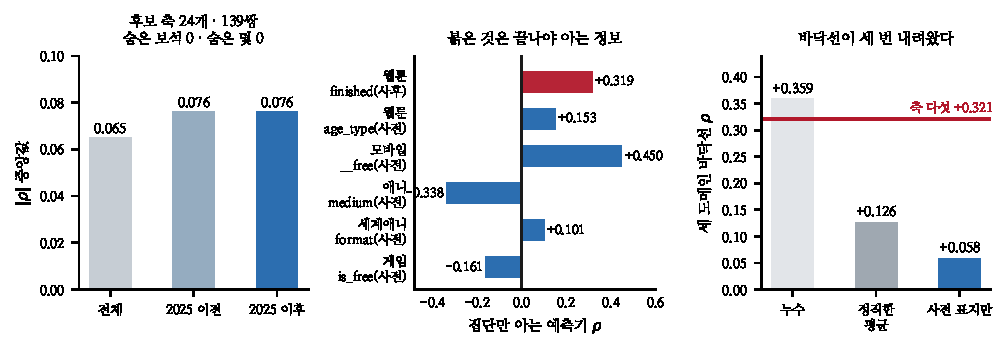
\includegraphics[width=\textwidth]{figs/when.pdf}
\caption{왼쪽 --- 후보 축을 기간 갈라도 숨은 것이 없다. 가운데 --- 붉은
것은 끝나야 아는 정보. 오른쪽 --- 바닥선이 세 번 내려왔다.}
\end{figure*}

\section{숨은 것은 없었다}

노트 140이 웹툰의 \texttt{goods\_scale}에서 ``전체 $+$0.033, 이전 $+$0.378,
이후 $-$0.283''을 찾고 나서, 노트 116이 전체 상관으로 걸러 낸 후보 축들에도
그런 구조가 있을 것이라 봤다. 스물네 개를 도메인별로 기간 갈라 다시 쟀다
(139쌍).

\begin{table}[t]
\centering\tsize
\caption{후보 축 재검토. 139쌍.}
\begin{tabular}{lr}
\toprule
숨은 보석 (전체 $<$.10, 두 기간 $\ge$.18 같은 부호) & \textbf{0} \\
숨은 덫 (전체 $\ge$.15, 기간 부호 반대) & \textbf{0} \\
부호 다름 (둘 다 $|\rho|\ge$.08) & 4 (3\%) \\
$|\rho|$ 중앙 --- 전체 / 이전 / 이후 & .065 / .076 / .076 \\
\bottomrule
\end{tabular}
\end{table}

\claimx{\textbf{전체 상관은 97\%의 경우 멀쩡하다.} 노트 140이 ``축 요약에
전체 상관을 쓰지 않는다''를 규약으로 세웠는데, 그 근거는 웹툰
\texttt{goods\_scale} 한 쌍이었다. 139쌍을 보니 그 정도 구조는
3\%다.}{그래도 규약은 남긴다 --- 3\%가 하필 결과를 뒤집는 자리에 있었다.
비용이 싸니 기간 갈라 보는 편이 낫다. \textbf{다만 ``전체 상관은 믿을 수
없다''는 과장이었다.}}

\section{대신 다른 것이 나왔다}

훑기의 상위에 \texttt{kitsu\_rank}와 \texttt{kitsu\_rating}이 있었다.
세계애니에서 전체 $+$0.410 · 이전 $+$0.415 · 이후 $+$0.391로 안정적이다.
붙여 보니 부스팅의 판이 $+$0.3363에서 $+$0.3811로 \textbf{$+$0.045} 오른다.

\claimx{\textbf{그리고 누수 가드 둘을 모두 통과한다.} 라벨 상관 0.41이
문턱 0.70 아래이고, Kitsu는 라벨을 만든 AniList와 다른 플랫폼이다. 노트
117이 세운 두 층이 이것을 못 막는다.}{노트 117의 두 층은 ``라벨의 복사본''
을 막는 장치였고, 이것은 복사본이 아니라 \emph{다른 곳에서 잰 같은 것}이다.}

\claimx{\textbf{그런데 쓰면 안 된다 --- 시점 때문이다.} Kitsu 필드는
전부 지금 긁은 스냅샷이다(현재 평점 · 현재 순위 · 현재 사용자 수). 작품이
나오기 전에는 존재하지 않으므로, 기획 단계에서 쓸 수 없다.}{하네스의 시간
분할은 \emph{레코드의} 시점만 본다 --- 축 값이 언제 측정됐는지는 안 본다.
그래서 사후 축이 시간 마스크를 그냥 통과한다.}

\section{그 잣대를 내 것에 댔다}

\begin{table}[t]
\centering\tsize
\caption{집단 표지의 시점. 같은 방식으로 잰 바닥선.}
\begin{tabular}{llr}
\toprule
& 시점 & $\rho$ \\
\midrule
\textbf{웹툰 finished} & \textbf{사후} & \textbf{$+$.319} \\
웹툰 age\_type & 사전 & $+$.153 \\
모바일 가격 & 사전 & $+$.450 \\
애니 매체 & 사전 & $-$.338 \\
세계애니 포맷 & 사전 & $+$.101 \\
게임 무료 여부 & 사전 & $-$.161 \\
\bottomrule
\end{tabular}
\end{table}

\claimx{\textbf{노트 138의 헤드라인이 뒤집힌다.} ``플래그 하나가 축 다섯을
이긴다''의 그 플래그는 웹툰의 완결 여부이고, 완결 여부는 \emph{끝나야
안다.} 사전에 아는 연령등급으로 바꾸면 $+$0.319가 $+$0.153이 되고
축 다섯($+$0.202)이 이긴다.}{연령등급이 완결 여부만큼 좋은 표지라는
뜻은 아니다 --- 사전에 아는 것 중 제일 나은 것을 더 찾아볼 여지가 있다.}

\begin{table}[t]
\centering\tsize
\caption{세 도메인 바닥선이 세 번 내려왔다.}
\begin{tabular}{lrl}
\toprule
& $\rho$ & 무엇이 틀렸나 \\
\midrule
노트 138 첫판 & $+$.3589 & 검정 집합 평균 (누수) \\
노트 138 고침 & $+$.1255 & 학습 평균, 사후 표지 \\
\textbf{노트 141} & \textbf{$+$.0583} & 사전 표지만 \\
\midrule
축 다섯 (참고) & $+$.3208 & \\
\bottomrule
\end{tabular}
\end{table}

\claimx{\textbf{세 번 다 같은 방향이었다.} 바닥선을 만들 때마다 예측 시점에
없는 정보를 썼고, 그때마다 바닥선이 실제보다 높게 나와 모형이 못해 보였다.
사전 정보만 쓰면 축 다섯($+$0.321)이 바닥선($+$0.058)을 크게
이긴다.}{바닥선이 낮아졌다고 모형이 좋아진 것은 아니다. 달라진 것은
``무엇과 견주는가''뿐이다.}

\section{가드 열째 --- 시점}

\texttt{lab/provenance.py}에 축마다 시점을 적었다. 사전 · 사후 · 정적
셋이고, \textbf{등록 안 된 축은 사후로 본다} --- 두 번 다 모르는 채로
통과했으니 모르면 막는 쪽이 맞다.

\begin{table}[t]
\centering\tsize
\caption{누수 가드 세 층.}
\begin{tabular}{lll}
\toprule
& 막는 것 & 노트 \\
\midrule
① 라벨 상관 & 라벨의 복사본 & 117 \\
② 출처 플랫폼 & 라벨을 만든 계수기 & 117 \\
\textbf{③ 측정 시점} & \textbf{나중에 잰 것} & \textbf{141} \\
\bottomrule
\end{tabular}
\end{table}

현행 축 세트를 훑으니 \texttt{trendcal} 열아홉 축이 전부 사전/정적이고,
Kitsu 축을 붙이면 곧바로 걸린다. 웹툰 집단 표지는 연령등급으로 갈아 끼웠다.

\begin{table}[t]
\centering\tsize
\caption{남은 것.}
\begin{tabular}{ll}
\toprule
사전 표지 & 웹툰에 더 나은 사전 표지가 있나 \\
후보 축 & 정적으로 분류한 것들의 실제 수집 시점 확인 \\
바닥선 & 세 도메인 $+$.058 --- 다른 도메인도 재기 \\
\bottomrule
\end{tabular}
\end{table}

둘째 줄이 다음 자리다. 설명문 임베딩과 표지 특징을 ``정적''으로 분류했는데,
그 설명문과 표지를 \emph{언제} 긁었는지는 안 봤다. 연재 중에 갱신되는
소개글이라면 그것도 사후다.

\end{document}
